\chapter{Algorithms}

Dire qu'on va présenter deux algorithmes différents, mais qu'avant on explique l'extraction. Après on proposera deux petits algo pour accélerer la recherche de solution.

\section{Peaks extraction}

A \gls{cir} as presented in \ref{fig:cir_ex1} unfortunately does not exist in the real world, at least, not using the material presented in section \ref{loc_syst}. First, extra peaks will appears, due to the double, triple, etc...  reflection on the walls, on the furnitures of the room. Some peaks caused by diffraction may also appears. People walking or standing into the room will also modify the channel and so the \gls{cir}. Second, as previously stated in \ref{dwm1000}, the bandwidth of the DWM1000 is not infinite, occasioning a spatial extension of the different peaks. The evolution from a theoretical "perfect" case to a "real" one can be observed in Fig. \ref{fig:peaks_real}.

\begin{figure}[H]
\centering
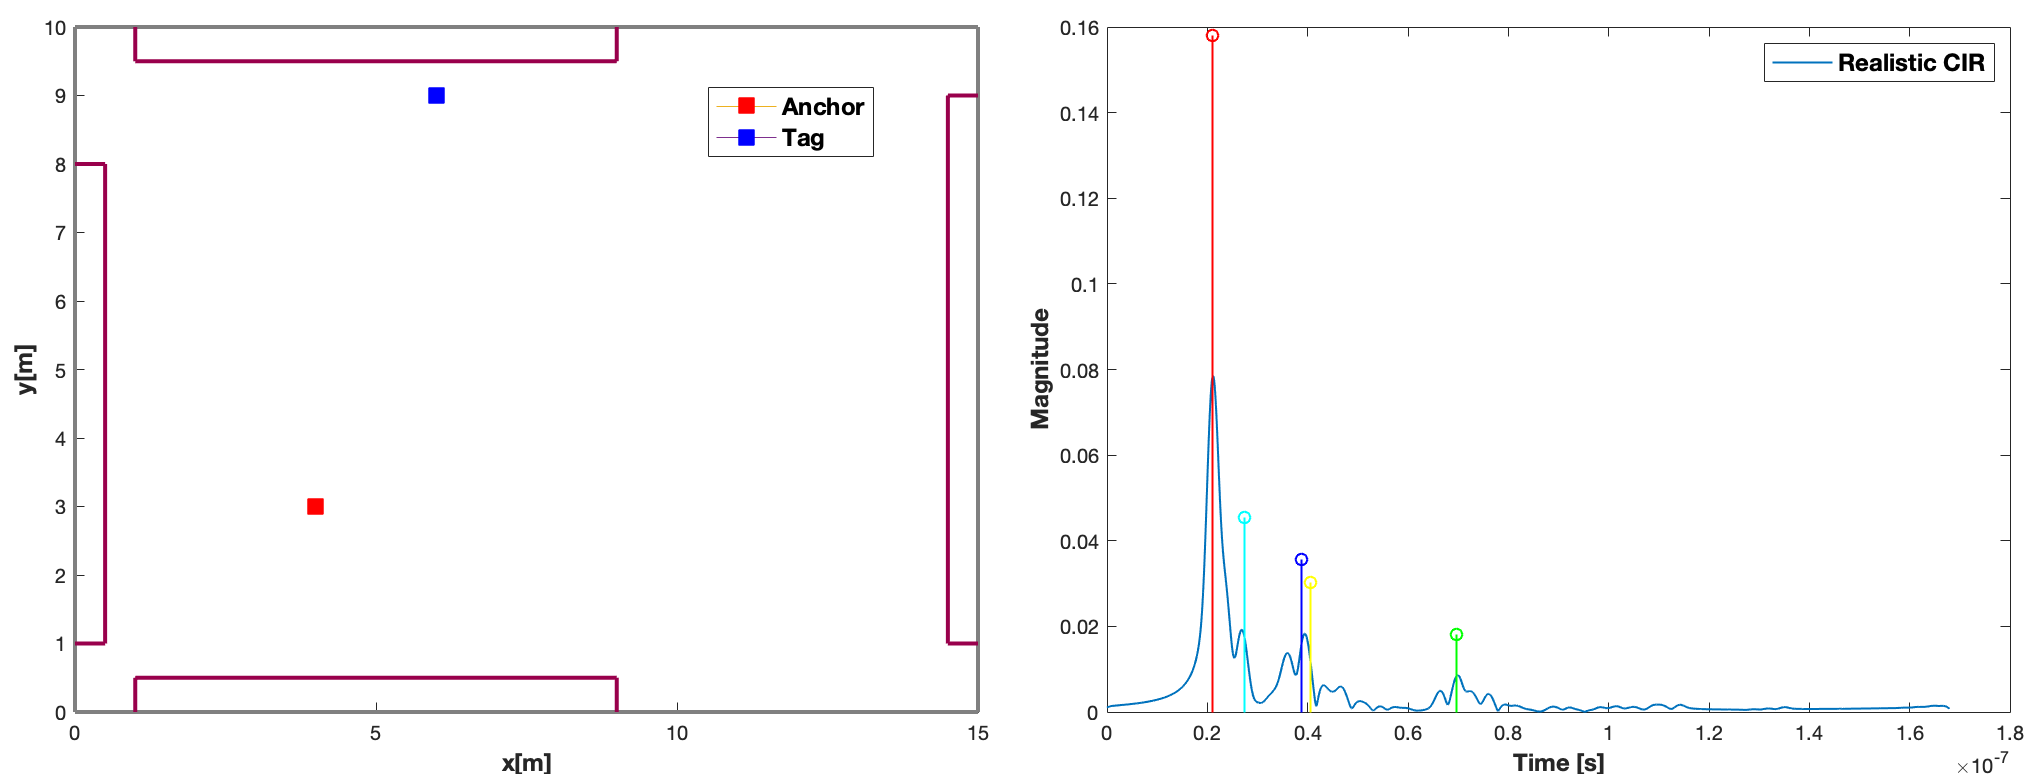
\includegraphics[width=\linewidth]{Images/cir_theo_real.png}
\caption{(Left) Room used to generate the realistic CIR using up to three reflected rays. (Right) Superposition of the CIR in Fig. \ref{fig:UWB_MPC_Theo} and the realistic CIR.\label{fig:peaks_real}}
\end{figure}

The simulation used to generate the realistic \gls{cir} is described in chapter \ref{simulations}. As one can observe, the peaks that originates from the theoretical case matches peaks in the realistic one. But one can also observe that some new peaks arises in the realistic ones, such as the ones around $0.4*10^{-7}s$. 
\vspace{2mm}

The goal of the peak extraction function is, as the name states, to extract the peaks matching the needs of the locating algorithm. As it will be seen in section \ref{hard_loc}, \ref{soft_loc}, the two methods do not achieve their objective in the same way, the optimal peaks will be slightly different. Hence the two different peaks extraction methods presented beneath.

\subsection{Soft case}

Expliquer la différence entre les deux algorithmes.

\subsection{Hard case}

In order to use the \gls{cir} recovered either in the simulation or from the experimental set-up, those need to be processed. The major objective is to retrieve the different peaks that originates from the physical anchor and the \glspl{va}. Unfortunately, the \gls{cir} obtained is not as simple as shown in Fig. \ref{fig:UWB_MPC_Theo}. In order to obtain the same results, one would need some antennas with an infinite bandwidth\footnote{In order to obtain Dirac peaks, one need an infinite bandwidth since the $\delta(t) \xrightarrow{\mathscr{F}} 1 $}, a "clean" room and to receive to the receiver side only the rays coming from the \gls{los} or reflected once.
\vspace{2mm}

\begin{figure}[H]
\centering
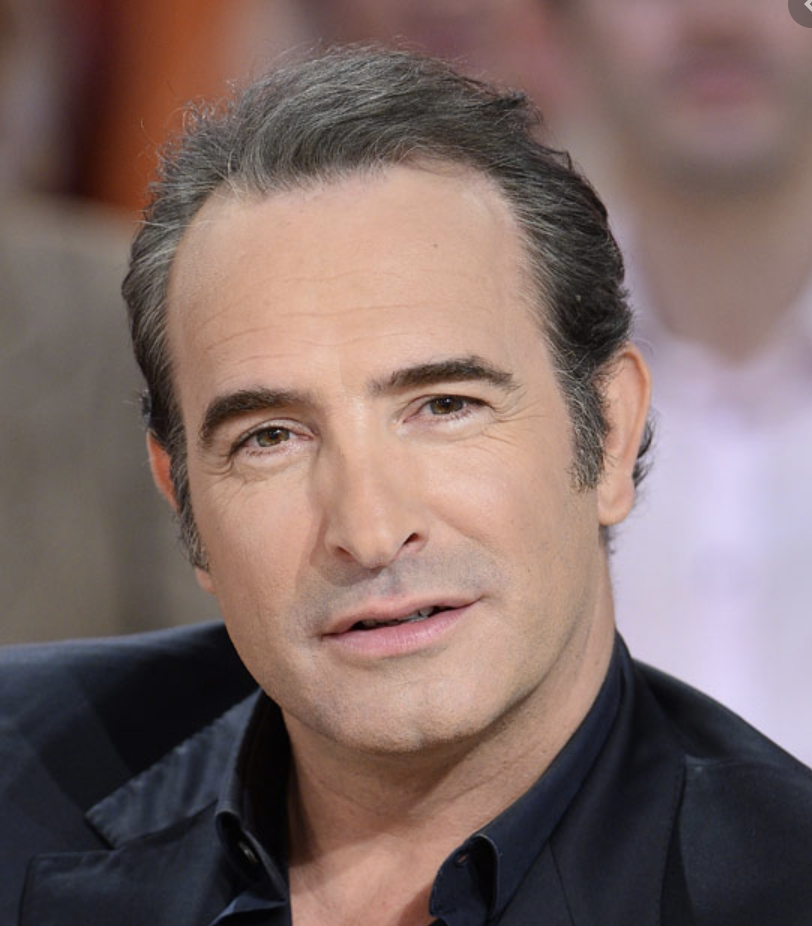
\includegraphics[width=.2\linewidth]{Images/Temporary_pic.png}
\caption{CIR example. \label{fig:cir_example}}
\end{figure}

The \gls{cir} shown for Fig. \ref{fig:cir_example} has been generated in a rectangular cluttered room of 15 over 10m, filled with furnitures. The selected bandwidth is the same as for the experimental set-up : 499.2MHz. The positions of the tag have been kept the same as in Fig. \ref{fig:cir_ex1}. As one can observe on Fig. \ref{cir}, getting the different peaks is not as trivial.
\vspace{2mm}

From the local maxima  of this \gls{cir}, only the most significant peaks should be extracted, since they likely are associated with the \gls{los} or first reflection. The parameter chosen to reflects the significance of a local maxima is its prominence.
\vspace{2mm}

The algorithm performs a search through the local maxima of the \gls{cir}. First the global maxima is considered as being the first peak corresponding to the \gls{los}. Hence only the local maxima arriving after are considered. Then, the rest of the local maxima are selected from the biggest to the shortest up to the point where $n$ peaks are chosen. All of those peaks are finally sorted based on the time associated with those peaks. 

The algorithm is formalized right beneath :
\vspace{2mm}

\begin{algorithm}[H]
 \KwData{$CIR$ such that $CIR(i)$ is a tuple $[time, val]$, $n \in \mathbb{N}$ the number of peaks requested}
 \KwResult{$Peaks$, ordered list of $n$ tuples.}
Initialization\;
$Peaks(1) \longleftarrow max(CIR)$\;
$CIR \longleftarrow CIR(max:end)$\;
$i \longleftarrow 2$\;
$r \longleftarrow 5$\;
 \While{$i <  n$ and $r < r_{max}$}{	
	\For{$el$ in $CIR$}{
    \If{$el > max(CIR)/r$}{
    $Peaks(i) \longleftarrow el$\;
    $i \longleftarrow i + 1$\;
    }
   }
   $r \longleftarrow r + 1$
 }
 $Order(Peaks)$
 \caption{Peaks Extraction \label{algo:peaks}}
\end{algorithm}

\section{Hard localization algorithm}
\label{hard_loc}
This locating system is based on the idea of trilateration and tries to mimic it. Using three peaks, it tries to match those with the anchor and two virtual anchors to find an intersection point as in the Fig. \ref{fig:triangulation}. Those three peaks are extracted with the algorithm \ref{algo:peaks} from the received \gls{cir} at the tag. As briefly explained is section \ref{loc_syst_mpc}, there is two main difference with the theoretical case.

\subsection{Virtual antennas combination}

The hypothesis that the greatest peak corresponds to the one from the \gls{los} ray is made. Concerning the second a third peak, since each one can not be surely associated with a \gls{va}, the only available solution is to try every combination of \glspl{va}. The order being important\footnote{Associating the tuple $(d_1, d_2)$ to $(va_1, va_2)$ is not equivalent to associate it to $(va_2, va_1)$.}, it is $P^2_4 = \frac{4!}{2!} = 12$ different systems to solve. This computation has been made for a room with a simple geometry, a rectangular, four walls room in this case, of course with a more complex geometry, the number of possible combination would increase.
\vspace{2mm}

On Fig. \ref{fig:va_sym}, a possible problem is shown. The \gls{cir} shown on the left side is obtained by computing only the \gls{los} and the first reflections onto the different walls. In theory, five different peaks should be seen, but only four appears. In this particular case, the second peak is formed by the peaks from $VA_1$ and $VA_2$, which will be undistinguishable.

\begin{figure}[H]
\centering
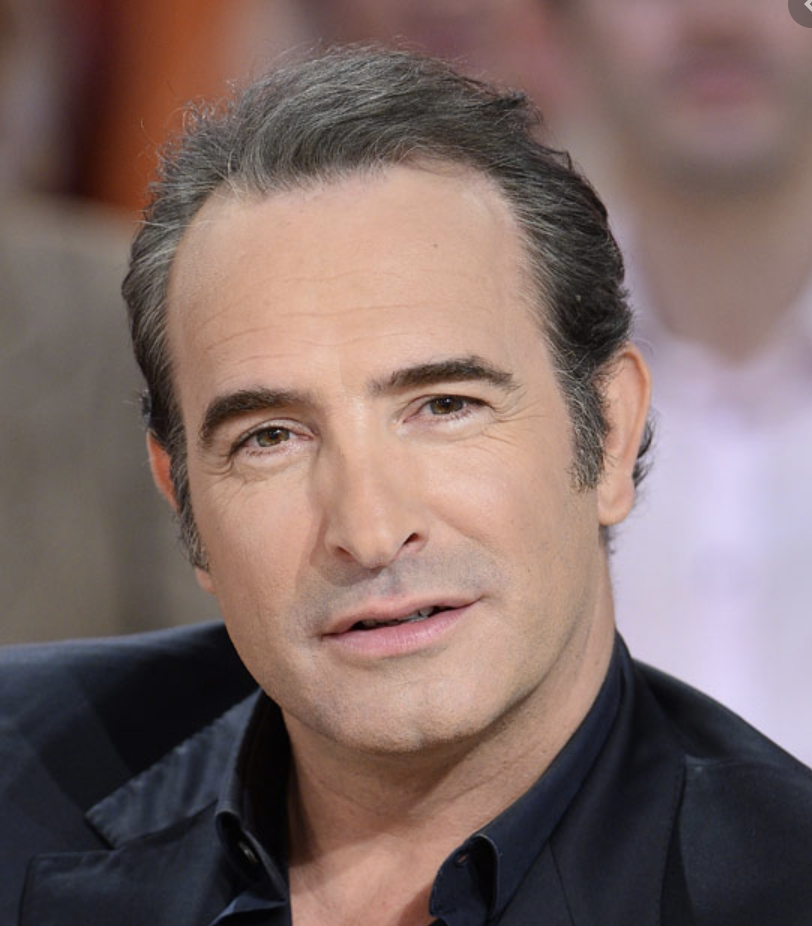
\includegraphics[width=.2\linewidth]{Images/Temporary_pic.png}
\caption{Map left, CIR right = montrer la sym \label{fig:va_sym}}
\end{figure}

What could happen in that case is that the peaks taken from the \gls{cir} could not correspond to some actual theoretical peaks\footnote{The one that corresponds to one reflection. }. Such an example can be seen on Fig. \ref{fig:va_sym} where the third orange peak does not correspond to any theoretical peak. To overcomes this problem, the proposed solution is to consider the cases peaks are mingled. Hence to the twelve possibles combinations, one would have to consider that the second orange peak originate from two different \gls{va}.
\vspace{2mm}

This method has the drawback of requiring much computation since twelve more peaks - \glspl{va} needs to be checked, but it will solve some symmetry-related problem. This kind of problem mostly occurring on the brown line on the map, being the axial symmetry between the two \gls{va}. Since this problem only occurs in those specific cases, one should first check the original antenna combination before checking those added one.
\vspace{2mm}

Another source of troubles for this algorithm is due to the finite bandwidth of the antennas. As it can be seen on Fig. \ref{fig:inftofin}, peaks that can be distinguished on the left \gls{cir} are mingled in the right \gls{cir}. This phenomena can be observed with the green peaks for example.

\begin{figure}[H]
\centering
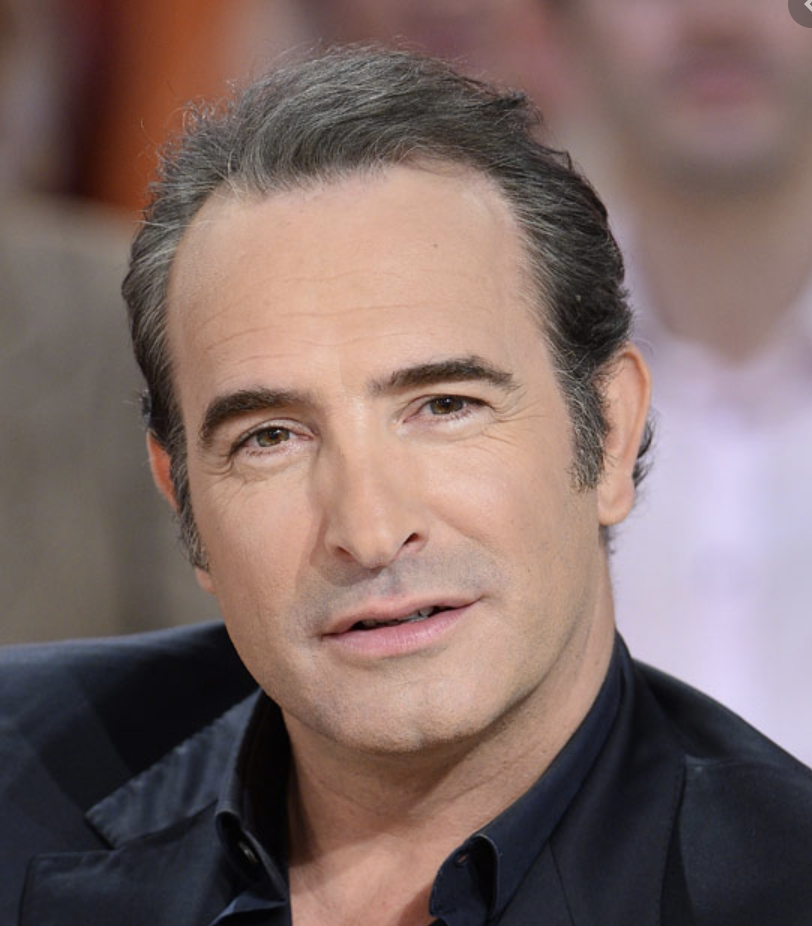
\includegraphics[width=.2\linewidth]{Images/Temporary_pic.png}
\caption{Comparison between an infinite BW CIR and a finite one \label{fig:inftofin}}
\end{figure}

To deal with this problem, the solution proposed is the same as the one dealing with the mingled peaks. The precision achieved on the localization in such case would be reduced  in those cases. Such examples will be shown in chapter \ref{simulations}.
\vspace{2mm}

\subsection{System solver}

Those systems are solved one at a time, starting with the twelve 'basic' ones, pursuing with the particular cases presented above. Since there is almost zero chances that the system leads into a perfect one point solution, the system \ref{eq:syst_exact} can not be simply resolved. The three equations are solved two by two, giving six real or complex solutions. From this point, the algorithm first exclude the solutions lying outside of the room, the solutions having a too big imaginary part are also discarded\footnote{The notion of "too big" is completely subjective. It appears that when two circle are close to have an intersection, the imaginary part is smaller. \color{red} NEED A PROOF \color{black}}. 
\vspace{2mm}

Using the remaining solutions, the algorithm needs to check if those can be combined to retrieve a suitable solution. A solution is considered as suitable if the algorithm can find three solutions being relatively close to each other. This notion of "relatively close" is subjective and is one of the parameter that one can vary to tune the algorithm. If no solution is found using all the combinations, then no location is provided, hence the qualification of "hard".
\vspace{2mm}

- Mettre le schéma de l'antenne qui est dans un coin, et des 4 zones qui se dessinent
- Expliquer qu'on va tester toutes les possibilités 2 à 2, mais qu'on peut éliminer certaines avec l'algo speed 2.

\section{Soft localization algorithm}
\label{soft_loc}

\subsection{CIR MSE}

Pour la forme de la CIR, bien expliquer pourquoi ça ne marche pas vraiment. Même en atténuant les autres pics de la même manière que le pic principal. Parce que la réponse qu'on reçoit peut avoir un LoS légèrement plus obstrué que le reste, ou vice versa. Ca marche bien dans la simulation, mais ça sera probablement moins efficace IRL.

\subsection{Time MSE}

Méthode préférée à CIR

\section{Speed-Up Algorithms}
\label{speed-up}
\subsection{Speed-Up 1}

The aim of this algorithm is to speed up the locating process by reducing the number of needed computations. To achieve this, the \gls{cir}, that needs to be computed at each location, is only computed in a reduced set of possible position for the tag.
\vspace{2mm}

Using the \gls{sdstwr}, the \gls{tof} of the signal between the tag and the anchor can be computed\footnote{In the simulation, it will be assumed to be extracted from the \gls{cir}}. Based on this \gls{tof}, a circle can be traced with the center on this anchor and the radius being the estimated distance deduced from the \gls{tof}. In theory, the tag is supposed to be located on this circle, but due to the discretization and errors on the \gls{tof}, a margin is taken to get the set of possible locations. This margin resides in the two orange circles, that can be observed on Fig. \ref{fig:speedup_1}.
\vspace{2mm}

\begin{figure}[H]
\centering
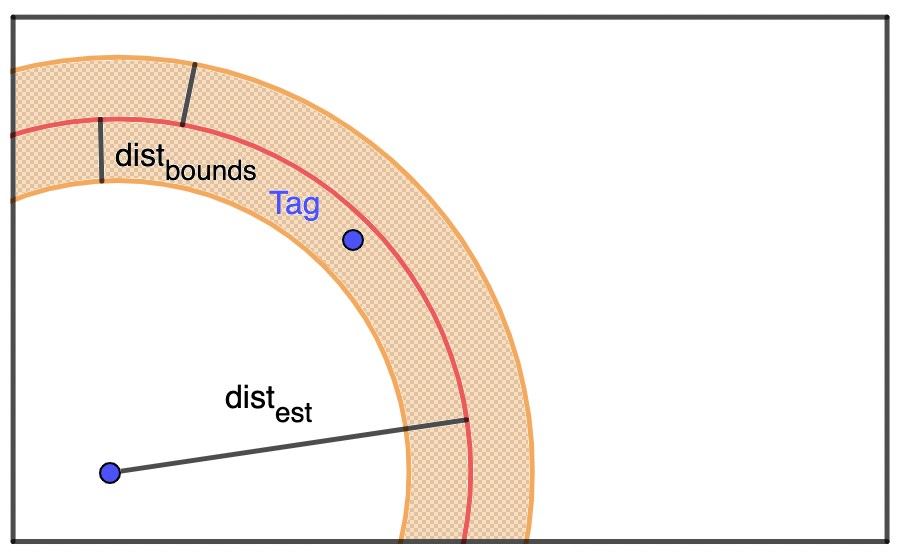
\includegraphics[width=.65\linewidth]{Images/algo_1.png}
\caption{Example of algo 1}
\label{fig:speedup_1}
\end{figure}

From the position inside those boundaries, a mask matrix representing all the position of the room is filled with ones for the position inside of the orange zone. The other positions are left to zero. Later, this mask is used to reduce the computations since only the values associated with a one will be tested.

\subsection{Speed-Up 2}

Choix des ancres en utilsant l'algorithme numéro 1


